\chapter{\label{chap:stats}Statistics (for computational linguists)}

Statistics is considered to be ``the language of science'' by many.
Any experimental or observational result in science has to be
filtered through statistical procedures for their reliability.
To be more scientific or rational,
business or political decision made in industry or government
has to be justified by statistics.

\emph{Descriptive statistics} consist of tools and methods
for summarize and visualizing data.
It allows us to understand, or `make sense of', the data.
In contrast, the aim of \emph{Inferential statistics} is
to make inferences about a large, possibly infinite,
\emph{population} of objects from a \emph{sample} taken from the population.
In many ways,
inferential statistics share the same theory and methods with
\emph{machine learning},
which is an essential part of virtually any method or tool used
in modern computational linguistics and natural language processing.
The difference between (inferential) statistics and machine learning is
the way the results from these (common) theory and methods are used.
In machine learning,
build and tune models using available data and utilize the model unseen data.
For example,
given an annotated corpus with named entities,
we may want to build a \emph{named entity recognizer} that can be used for spotting them in unlabeled texts we want to process.
In statistics as used typically in many fields of research,
we want to get conclusions a population based on
a model whose parameters are estimated using a sample from this population.
For example,
we may want to predict the results of an upcoming elections based on
a poll administered on a small fraction of the electorate in the country.

Although aims and approaches differ,
a good understanding of statistics is invaluable for machine learning.
Furthermore,
computational linguistics is largely a experimental field,
we often test our theories and methods on corpora
or use other experimental methods.
In such experiments,
a basic question is the reliability of the results outside
the corpora (sample) used in the study.
The methods for answering this question is part of the 
statistics used in many experimental research.

In this chapter,
after brief section on descriptive statistics,
we will discuss some of the foundational topics
in the (classical) inferential statistical methods,
and also discuss some methods that are particularly useful
in computational linguistics experiments.

\section{Descriptive statistics}

We have seen some of the relevant concepts
in Chapter~\ref{chap:prob} already.
\emph{Mean}, \emph{median} and \emph{mode} are useful quantities
indicating central tendency. 
\emph{Variance} and \emph{standard deviation} are
measures of variation or dispersion.
\emph{Correlation coefficient} we have discussed shows
linear dependence within a bivariate data set.
These all are important characteristics of a given data set.
Instead of looking through tens, thousands or billions of raw data points,
we get much more information by looking at these \emph{summary statistics}.

However, it is always a good idea to visualize the data,
since the summary statistics can be quite similar
for data that differ in important ways.
Descriptive statistics provide a set of conventional plots that allow us
to quickly see other properties of data.
For example \emph{histograms} allow us to visualize the data
where we can seem much more than the above statistics.
For example, besides the central tendency and variation,
we can also see easily the \emph{range} and \emph{skewness} of the data.
Another conventional plot, \emph{box and whisker plots},
or simply \emph{box plots},
also show similar information in a more concise manner.
They are often useful to plot the side-by-side
for numeric data based on some categorical \emph{covariate}.
For bivariate data,
\emph{scatter plots} are very useful for observing
both variables and their relation.
We will not explain these statistics or graphical tools in detail here.
Below,
we will only go thorough some of them
with examples from a contrived educational data set.
It is important to understand them,
since, like any other field of research,
we will often use these while working with linguistic data.

\begin{marginfigure}
  \tikzsetnextfilename{anscombe-scatter}%
  \begin{tikzpicture}
    % The data is copied from Wikipedia:
    % <https://en.wikipedia.org/wiki/Anscombe's_quartet>
    \pgfplotstableread{
			x1			y1		 x2		 y2		 x3		  y3     x4     y4
			10.0 	 8.04 	10.0 	9.14 	10.0 	 7.46 	 8.0 	 6.58
			 8.0 	 6.95 	 8.0 	8.14 	 8.0 	 6.77 	 8.0 	 5.76
			13.0 	 7.58 	13.0 	8.74 	13.0 	12.74 	 8.0 	 7.71
			 9.0 	 8.81 	 9.0 	8.77 	 9.0 	 7.11 	 8.0 	 8.84
			11.0 	 8.33 	11.0 	9.26 	11.0 	 7.81 	 8.0 	 8.47
			14.0 	 9.96 	14.0 	8.10 	14.0 	 8.84 	 8.0 	 7.04
			 6.0 	 7.24 	 6.0 	6.13 	 6.0 	 6.08 	 8.0 	 5.25
			 4.0 	 4.26 	 4.0 	3.10 	 4.0 	 5.39 	19.0 	12.50
			12.0 	10.84 	12.0 	9.13 	12.0 	 8.15 	 8.0 	 5.56
			 7.0 	 4.82 	 7.0 	7.26 	 7.0 	 6.42 	 8.0 	 7.91
			 5.0 	 5.68 	 5.0 	4.74 	 5.0 	 5.73 	 8.0 	 6.89
    }{\anscombe};
    \begin{groupplot}[%
      group style={
          group name=my plots,
          group size=1 by 4,
          xlabels at=edge bottom,
          xticklabels at=edge bottom,
          vertical sep=3mm,
      },
      ticklabel style={font=\tiny},
      xlabel style={font=\scriptsize,
         at=(current axis.south east), anchor=south east},
      ylabel style={font=\scriptsize,
         at=(current axis.north west),
         anchor=north west, rotate=-90},
      title style={yshift=-3ex,font=\scriptsize},
      x=2mm,y=2mm,
      xmin=4, xmax=20,
      ymin=3, ymax=14,
      major tick length=0.5mm,
      minor tick length=0.2mm,
      enlarge x limits=true,
      enlarge y limits=true,
      clip=false,
      xlabel=$x$, ylabel=$y$,
    ]
        \nextgroupplot
        \addplot[mark=*,mark size=1pt,only marks,blue]
          table[x=x1,y=y1] {\anscombe};
        \node[font=\small,anchor=south west] at (axis description cs:1,0) {(a)};

        \nextgroupplot
        \addplot[mark=*,mark size=1pt,only marks,blue]
          table[x=x2,y=y2] {\anscombe};
        \node[font=\small,anchor=south west] at (axis description cs:1,0) {(b)};

        \nextgroupplot
        \addplot[mark=*,mark size=1pt,only marks,blue]
          table[x=x3,y=y3] {\anscombe};
        \node[font=\small,anchor=south west] at (axis description cs:1,0) {(c)};

        \nextgroupplot
        \addplot[mark=*,mark size=1pt,only marks,blue]
          table[x=x4,y=y4] {\anscombe};
        \node[font=\small,anchor=south west] at (axis description cs:1,0) {(d)};
    \end{groupplot}
  \end{tikzpicture}
  \caption{\label{fig:anscombe-scatter}%
    Scatter plots of Anscombe's quartet.
  }
\end{marginfigure}
A famous data set where many descriptive statistics agree
despite important differences is called Anscomebe's quartet,
which consists of four paired sets of real numbers.
All three data sets have the same or very similar
(same up to 2 or more significant digits)
means ($\mu_{x} = 9$, $\mu_{y} = 7.50$) and variances
($\sigma^{2}_{x} = 11$, $\sigma^{2}_{y} = 4.125$),
as well as the correlation coefficient ($r = 0.816$) between $x$ and $y$.
Although one could conclude from these (otherwise useful) summary statistics
that the data sets are very similar,
visualizing them shows quite a different story.
The differences are most striking in scatter plots presented in 
Figure~\ref{fig:anscombe-scatter}.

\begin{figure}
  \tikzsetnextfilename{anscombe-histogram}%
  \begin{tikzpicture}
    \pgfplotstableread{
			x1			y1		 x2		 y2		 x3		  y3     x4     y4
			10.0 	 8.04 	10.0 	9.14 	10.0 	 7.46 	 8.0 	 6.58
			 8.0 	 6.95 	 8.0 	8.14 	 8.0 	 6.77 	 8.0 	 5.76
			13.0 	 7.58 	13.0 	8.74 	13.0 	12.74 	 8.0 	 7.71
			 9.0 	 8.81 	 9.0 	8.77 	 9.0 	 7.11 	 8.0 	 8.84
			11.0 	 8.33 	11.0 	9.26 	11.0 	 7.81 	 8.0 	 8.47
			14.0 	 9.96 	14.0 	8.10 	14.0 	 8.84 	 8.0 	 7.04
			 6.0 	 7.24 	 6.0 	6.13 	 6.0 	 6.08 	 8.0 	 5.25
			 4.0 	 4.26 	 4.0 	3.10 	 4.0 	 5.39 	19.0 	12.50
			12.0 	10.84 	12.0 	9.13 	12.0 	 8.15 	 8.0 	 5.56
			 7.0 	 4.82 	 7.0 	7.26 	 7.0 	 6.42 	 8.0 	 7.91
			 5.0 	 5.68 	 5.0 	4.74 	 5.0 	 5.73 	 8.0 	 6.89
    }{\anscombe};
    \begin{groupplot}[%
      group style={
          group name=my plots,
          group size=4 by 2,
          xlabels at=edge bottom,
          xticklabels at=edge bottom,
          horizontal sep=3mm,
          vertical sep=3mm,
      },
      ticklabel style={font=\tiny},
      xlabel style={font=\scriptsize, yshift=1ex},
      ylabel style={font=\scriptsize},
      title style={yshift=-3ex,font=\scriptsize},
      x=1.2mm,y=2mm,
      xmin=4, xmax=20,
      ymin=0, ymax=10,
      major tick length=0.5mm,
      minor tick length=0.2mm,
      enlarge x limits=true,
      enlarge y limits=true,
      clip=false,
      ybar,
      axis x line*=bottom,
    ]

        \nextgroupplot[axis y line*=left,
                       tick align=outside,
                       xlabel=$x$,
        ] 
        \addplot +[hist =  {
                    bins=6,
                    data min=4,
                    data max=20,
                   },
                   fill=blue!20,
          ] table [y index=0] {\anscombe};
        \node[font=\small,anchor=south] at (axis description cs:0.5,1) {(a)};

        \nextgroupplot[%
                       axis y line=none,
                       xlabel=$x$,
        ]
        \addplot [hist =  {
                    bins=6,
                    data min=4,
                    data max=20,
                   },
                   fill=blue!20,
          ] table [y index=2] {\anscombe};
        \node[font=\small,anchor=south] at (axis description cs:0.5,1) {(b)};

        \nextgroupplot[%
                       axis y line=none,
                       xlabel=$x$,
        ]
        \addplot [hist =  {
                    bins=6,
                    data min=4,
                    data max=20,
                   },
                   fill=blue!20,
          ] table [y index=4] {\anscombe};
        \node[font=\small,anchor=south] at (axis description cs:0.5,1) {(c)};


        \nextgroupplot[%
                       axis y line*=right,
                       xlabel=$x$,
        ]
        \addplot [hist =  {
                    bins=6,
                    data min=4,
                    data max=20,
                   },
                   fill=blue!20,
          ] table [y index=6] {\anscombe};
        \node[font=\small,anchor=south] at (axis description cs:0.5,1) {(d)};
                   
        %% y
        \nextgroupplot[axis y line*=left,
                       tick align=outside,
                       xlabel=$y$,
        ] 
        \addplot +[hist =  {
                    bins=6,
                    data min=4,
                    data max=20,
                   },
                   fill=blue!20,
          ] table [y index=1] {\anscombe};

        \nextgroupplot[%
                       axis y line=none,
                       xlabel=$y$,
        ] 
        \addplot [hist =  {
                    bins=6,
                    data min=4,
                    data max=20,
                   },
                   fill=blue!20,
          ] table [y index=3] {\anscombe};

        \nextgroupplot[%
                       axis y line=none,
                       xlabel=$y$,
        ]
        \addplot [hist =  {
                    bins=6,
                    data min=4,
                    data max=20,
                   },
                   fill=blue!20,
          ] table [y index=5] {\anscombe};

        \nextgroupplot[%
                       axis y line*=right,
                       xlabel=$y$,
        ] 
        \addplot [hist =  {
                    bins=6,
                    data min=4,
                    data max=20,
                   },
                   fill=blue!20,
          ] table [y index=7] {\anscombe};
                   
    \end{groupplot}
  \end{tikzpicture}
  \caption{
    Histograms of components of Anscombe's quartet.
  }\label{fig:anscombe-histogram}%
\end{figure}

Besides the scatter plots
which are very useful for visualizing bivariate data,
there are a number of other conventional plots for univariate data.
Probably most common one is histograms,
where data is split into fixed-interval bins,
and the number of data points in each bin is displayed as
a box whose height is proportional to the number of data points
in the interval.
Histograms show the shape of the probability distributions functions.
Figure~\ref{fig:anscombe-histogram} shows the histograms of both $x$ and $y$
variables for all four data sets in the Anscombe's quartet.
Although not as striking as the scatter plots,
it is also clear from these graphs
that the data is not the same despite same or similar summary statistics.

\begin{marginfigure}
  \tikzsetnextfilename{anscombe-boxplot}%
  \begin{tikzpicture}
    \pgfplotstableread{
			x1			y1		 x2		 y2		 x3		  y3     x4     y4
			10.0 	 8.04 	10.0 	9.14 	10.0 	 7.46 	 8.0 	 6.58
			 8.0 	 6.95 	 8.0 	8.14 	 8.0 	 6.77 	 8.0 	 5.76
			13.0 	 7.58 	13.0 	8.74 	13.0 	12.74 	 8.0 	 7.71
			 9.0 	 8.81 	 9.0 	8.77 	 9.0 	 7.11 	 8.0 	 8.84
			11.0 	 8.33 	11.0 	9.26 	11.0 	 7.81 	 8.0 	 8.47
			14.0 	 9.96 	14.0 	8.10 	14.0 	 8.84 	 8.0 	 7.04
			 6.0 	 7.24 	 6.0 	6.13 	 6.0 	 6.08 	 8.0 	 5.25
			 4.0 	 4.26 	 4.0 	3.10 	 4.0 	 5.39 	19.0 	12.50
			12.0 	10.84 	12.0 	9.13 	12.0 	 8.15 	 8.0 	 5.56
			 7.0 	 4.82 	 7.0 	7.26 	 7.0 	 6.42 	 8.0 	 7.91
			 5.0 	 5.68 	 5.0 	4.74 	 5.0 	 5.73 	 8.0 	 6.89
    }{\anscombe};

    \begin{groupplot}[%
      group style={
          group name=my plots,
          group size=2 by 1,
          xlabels at=edge bottom,
          xticklabels at=edge bottom,
          horizontal sep=3mm,
          vertical sep=3mm,
      },
      ticklabel style={font=\tiny},
      xlabel style={font=\scriptsize},
      ylabel style={font=\scriptsize},
      title style={yshift=-3ex,font=\scriptsize},
      x=4.5mm,y=1.2mm,
%      xmin=4, xmax=20,
      ymin=0, ymax=20,
      major tick length=0.5mm,
      minor tick length=0.2mm,
      enlarge x limits=true,
      enlarge y limits=true,
      clip=false,
      axis x line*=bottom,
    ]
      \nextgroupplot[%
        xtick={1,2,3,4},
        xticklabels={(a), (b), (c), (d)},
        boxplot/draw direction=y,
        axis y line*=left,
        xlabel=$x$,
      ]
      \addplot [
        boxplot prepared={
          lower whisker=4.0,
          lower quartile=6.5,
          median=9.0,
          upper quartile=11.5,
          upper whisker=14.0,
        },
        fill=blue!20,
        mark=*,mark size=1pt,
      ] coordinates {};
      \addplot [
        boxplot prepared={
          lower whisker=4.0,
          lower quartile=6.5,
          median=9.0,
          upper quartile=11.5,
          upper whisker=14.0,
        },
        fill=blue!20,
        mark=*,mark size=1pt,
      ] coordinates {};
      \addplot [
        boxplot prepared={
          lower whisker=4.0,
          lower quartile=6.5,
          median=9.0,
          upper quartile=11.5,
          upper whisker=14.0,
        },
        fill=blue!20,
        mark=*,mark size=1pt,
      ] coordinates {};
      \addplot [
        boxplot prepared={
          lower whisker=8.0,
          lower quartile=8.0,
          median=8.0,
          upper quartile=8.0,
          upper whisker=8.0,
        },
        fill=blue!20,
        mark=*,mark size=1pt,
      ] coordinates {(0,19)};

      \nextgroupplot[%
        xtick={1,2,3,4},
        xticklabels={(a), (b), (c), (d)},
        boxplot/draw direction=y,
        axis y line*=right,
        mark=*,mark size=1pt,
        xlabel=$y$,
      ]
      \addplot [
        boxplot prepared={
          lower whisker=4.260,
          lower quartile=6.315,
          median=7.580,
          upper quartile=8.570,
          upper whisker=10.840,
        },
        fill=blue!20,
        mark=*,mark size=1pt,
      ] coordinates {};
      \addplot [
        boxplot prepared={
          lower whisker=4.740,
          lower quartile=6.695,
          median=8.140,
          upper quartile=8.950,
          upper whisker=9.260,
        },
        fill=blue!20,
        mark=*,mark size=1pt,
      ] coordinates {(0,3.74)};
      \addplot [
        boxplot prepared={
          lower whisker=5.39,
          lower quartile=6.25,
          median=7.11,
          upper quartile=7.98,
          upper whisker=8.84,
        },
        fill=blue!20,
        mark=*,mark size=1pt,
      ] coordinates {(0,12.74)};
      \addplot [
        boxplot prepared={
          lower whisker=5.25,
          lower quartile=6.17,
          median=7.04,
          upper quartile=8.19,
          upper whisker=8.84,
        },
        fill=blue!20,
        mark=*,mark size=1pt,
      ] coordinates {(0,12.5)};
    \end{groupplot}
  \end{tikzpicture}
  \caption{\label{fig:anscombe-boxplot}%
    Box plots of components of Anscombe's quartet.
  }
\end{marginfigure}

Another common plot we briefly introduce here is \emph{box plot},
or \emph{box-and-whisker plots}.
Box plots,
display the middle two \emph{quartiles} around the median
which is indicated by a bar dividing the box.
When present,
the \emph{whiskers}, the lines extending from the box,
often extend until the lowest/highest data points
within \num[round-precision=1]{1.5} \emph{inter-quartile range} from the box
(although other conventions exist about what the whiskers represent).
The data outside these boundaries are considered \emph{outliers},
and plotted as separate dots.
Similar to histograms,
box plots show more than the central tendency and the variation.
As well as outliers,
the skewness of the distribution is often indicated by the box plots.
Box plots are particularly useful to compare multiple data series side-by-side.
Figure~\ref{fig:anscombe-boxplot} shows the box plots for $x$ and $y$ values in Anscombe's quartet.
Again,
they reveal that data has important differences
that mean and variances do not indicate.

In these notes,
we will limit our introduction/refresher of descriptive statistics 
to this short section.
However,
for readers who are not familiar with these concepts,
it is highly recommended to consult to the introductory material listed
at the end of the chapter.
These quantities/visualizations are not only useful for researchers,
they are also used everywhere in our modern societies,
hence, they are equally useful for any members of such societies.

\section{Population and the sample}


\section{Null hypothesis significance testing}

\begin{marginfigure}
  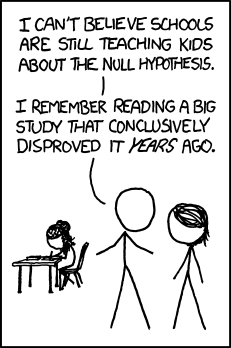
\includegraphics[width=\linewidth]{figures/xkcd-null_hypothesis}
  \caption{\url{http://xkcd.com/892/}: 
    Hell, my eighth grade science class managed to
    conclusively reject it just based on a classroom experiment.
    It's pretty sad to hear about million-dollar research teams
    who can't even manage that.
  }
\end{marginfigure}


\section*{Notes to self}

\begin{itemize}
  \item Read/cite \textcite{gigerenzer2007}
\end{itemize}
